\documentclass{beamer}
\usepackage{relsize}
\usepackage{color}

\usepackage{listings}
\usetheme{CambridgeUS}
%\usepackage{beamerthemesplit}  % new 
\usepackage{enumitem}
\usepackage{amsmath}                    % See geometry.pdf to learn the layout options. 
\usepackage{amsthm}                   % See geometry.pdf to learn the layout options. There 
\usepackage{amssymb}                    % See geometry.pdf to learn the layout options. 
\usepackage[utf8]{inputenc} 
\usepackage{graphicx}
\usepackage[english,bulgarian]{babel}

\lstset{language=C++,
                basicstyle=\ttfamily,
                keywordstyle=\color{blue}\ttfamily,
                stringstyle=\color{red}\ttfamily,
                commentstyle=\color{green}\ttfamily,
                morecomment=[l][\color{magenta}]{\#}
}

\newtheorem{mydef}{Дефиниция}[section]
\newtheorem{lem}{Лема}[section]
\newtheorem{thm}{Твърдение}[section]

\DeclareMathOperator{\restrict}{\upharpoonright}

\setitemize{label=\usebeamerfont*{itemize item}%
  \usebeamercolor[fg]{itemize item}
  \usebeamertemplate{itemize item}}

\setbeamercovered{transparent}



\begin{document}
\title[Увод в програмирането]{Типове, функции, граматики} 
\author{Калин Георгиев} 
\frame{\titlepage} 


\section{Типове} 


\begin{frame}
\centerline{Типове в езиците за програмиране}
\end{frame}



\begin{frame}[fragile]
\frametitle{Абстрактна необходимост}



\begin{itemize}
\item Моделиране
\pause
\item Различни физически характеристики на свойствата на реалните обекти
\pause
\item Физически и абстрактни свойства (тегло vs. име)

\end{itemize}

\pause


\begin{columns}[t]
  \begin{column}{0.4\textwidth}
\begin{itemize}
  \item Авто къща
  \item Авто морга
  \item Завод 
\end{itemize}

  \end{column}
  \begin{column}{0.6\textwidth}

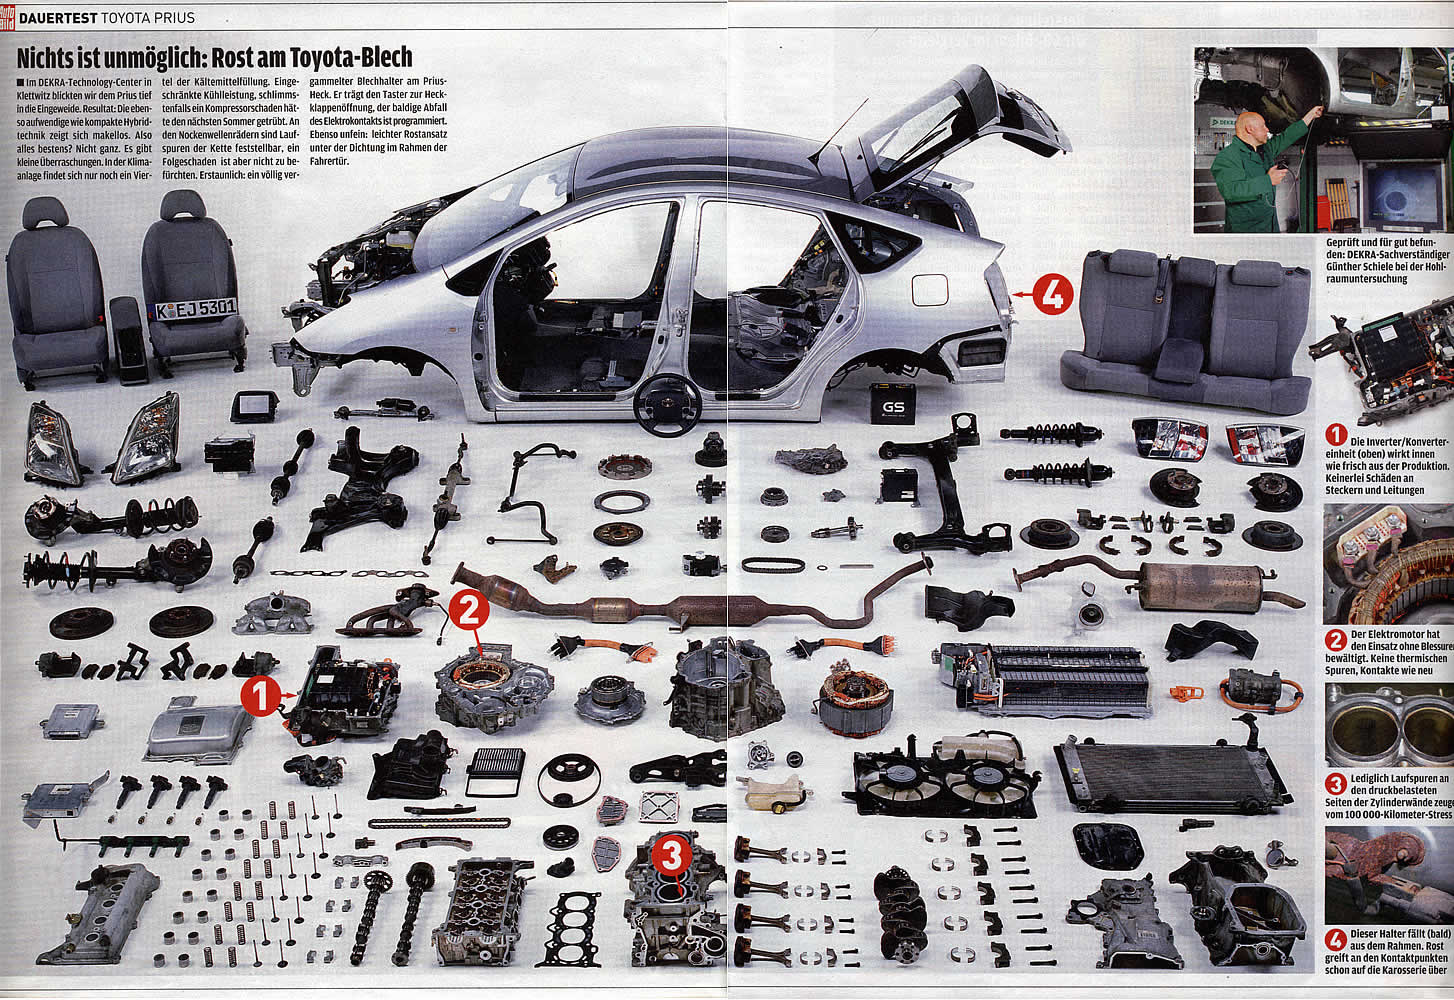
\includegraphics[width=6.4cm]{images/parts} 

  \end{column}
\end{columns}



\end{frame}


\begin{frame}[fragile]
\frametitle{Машинна необходимост}

\begin{itemize}
  \item Обем памет
\end{itemize}


\begin{tabular}{c c |c | c | c | c | c }
$127_{10}$= & 1 & 1 & 1& 1& 1& $1_{2}$ \\\hline

\end{tabular}

\begin{tabular}{c c |c | c | c | c | c | c }
$128_{10}$= & 1 & 0 & 0& 0& 0 & 0 & $0_{2}$ 
\end{tabular}
  
\pause

\begin{itemize}
  \item Приближено представяне на неизброими типове
\end{itemize}

$123.45 = \overbrace{12345}^{\textup{мантиса}}*\underbrace{10^{-2}}_{\textup{експонента}}$


\pause

\begin{itemize}
  \item Диапазон (range) vs. точност (precision)
  \pause
  \item Как представяме $1/3$
\end{itemize}


\end{frame}


\begin{frame}[fragile]
\frametitle{Примери}

\begin{flushleft}
\relscale{0.5}
\begin{lstlisting}
int main ()
{

  int int_a = 1, int_b = 2;
  double dbl_a = 1, dbl_b = 2;
  char chr_a = 'a', chr_b = 'b';


  cout << int_a / int_b << end;
  cout << dbl_a / dbl_b << end;
  cout << chr_a << end;

  int_a = 'a'; //int_a = chr_a;
  cout << int_a << end;

  char_a = 65;
  cout << chr_a << end;

  return 0;
}
\end{lstlisting}
\end{flushleft}

\end{frame}

\begin{frame}[fragile]
\frametitle{Математическа характеристика}


\textbf{Множество допустими стойности (Носител - $D$)}

\pause

\begin{itemize}
  \item Мъж, Жена
  \item 0..254
  \item $(\mathcal{R},\mathcal{R},\mathcal{R})$
\end{itemize}

\pause

\textbf{Операции}

\begin{itemize}
  \item $f:D\times D \rightarrow D$
  \item $f(x,y)=x+y$
\end{itemize}


\pause

\textbf{Предикати}

\begin{itemize}
  \item $p:D \rightarrow \{tt,ff\}$
  \item $p(x)=|x|_2==0$
\end{itemize}


\end{frame}


\section{Функции} 

\begin{frame}
\centerline{Функции. Подпрограми}
\end{frame}

\begin{frame}[fragile]
\frametitle{Функции в математиката}


\begin{itemize}
  \item Дефиниционна област (Domain)
  \item Множество на стойностите (Range) 
  \item $f:\mathbf{Domain} \rightarrow \mathbf{Range}$
\end{itemize}


\vspace{0.2cm}
$f(x) = x^2$

\begin{center}
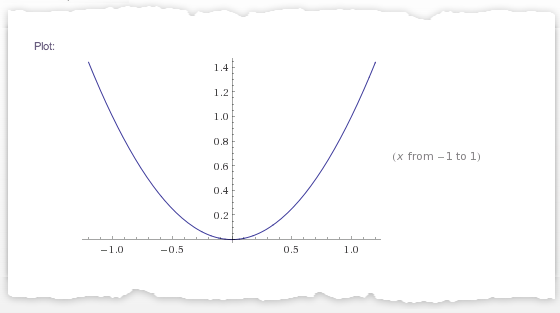
\includegraphics[width=7cm]{images/square}  
\end{center}


\end{frame}

\begin{frame}[fragile]
\frametitle{Функции в математиката}

$f(x,y) = x^2+y^2$

\begin{center}
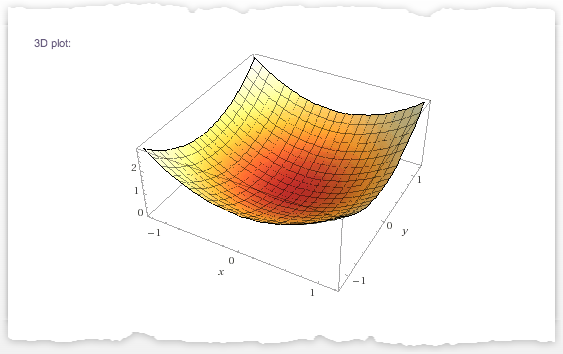
\includegraphics[width=7cm]{images/paraboloid}  
\end{center}

\end{frame}




\begin{frame}[fragile]
\frametitle{Подпрограми}

\begin{center}
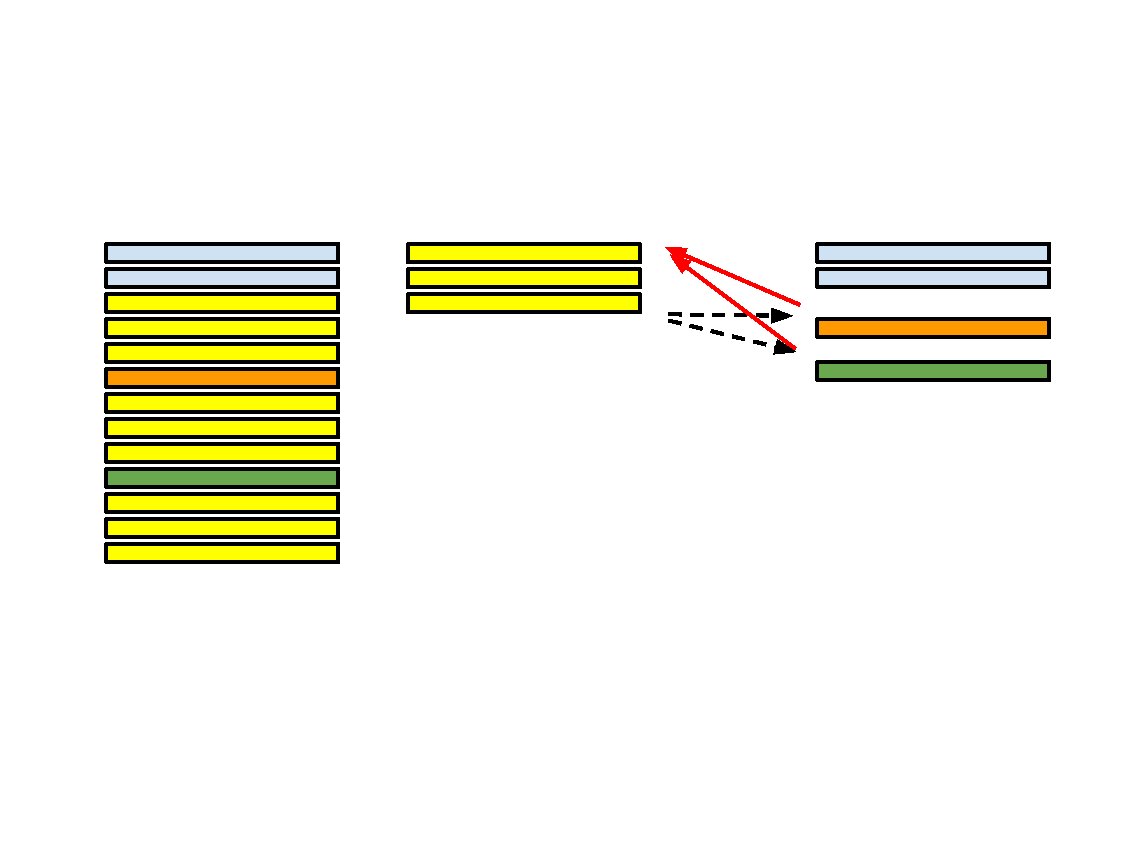
\includegraphics[width=7cm]{images/subprog}  
\end{center}


\end{frame}



\begin{frame}[fragile]
\frametitle{Лице на триъгълник по три страни}

\begin{flushleft}
\relscale{0.7}
$a,b,c \in \mathcal{R}$

$S = \sqrt{\frac{a+b+c}{2}\frac{b+c-a}{2}\frac{a+c-b}{2}\frac{a+b-c}{2}}=\sqrt{p(p-a)(p-b)(p-c)} \in \mathcal{R}$
\end{flushleft}

\pause

$s:\mathcal{R}\times\mathcal{R}\times\mathcal{R} \rightarrow \mathcal{R}$

\pause

$s(a,b,c)=\sqrt{p(p-a)(p-b)(p-c)}$


\end{frame}

\begin{frame}[fragile]
\frametitle{Съответната функция}

$s:\mathcal{R}\times\mathcal{R}\times\mathcal{R} \rightarrow \mathcal{R}$


$s(a,b,c)=\sqrt{p(p-a)(p-b)(p-c)}$


\begin{center}
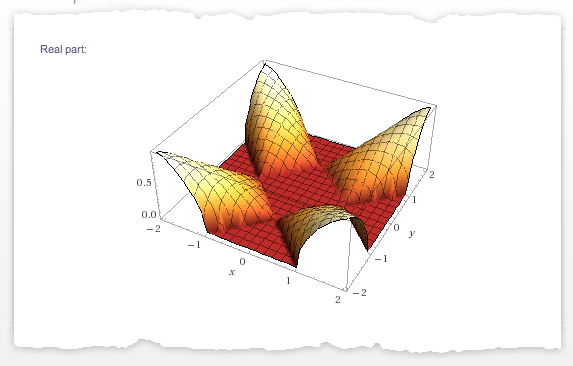
\includegraphics[width=6cm]{images/heron}  
\end{center}


\end{frame}
\begin{frame}[fragile]
\frametitle{Съответната подпрограма}

$s:\mathcal{R}\times\mathcal{R}\times\mathcal{R} \rightarrow \mathcal{R}$

$s(a,b,c)=\sqrt{p(p-a)(p-b)(p-c)}$

\pause

\begin{flushleft}
\relscale{0.5}
\begin{lstlisting}
double triangleSurface (double a, double b, double c)
\end{lstlisting}\pause\begin{lstlisting}
{
  double p = (a+b+c)/2;
  double surface = sqrt (p*(p-a)*(p-b)*(p-c));

  return surface;
}
\end{lstlisting}
\end{flushleft}


\end{frame}

\begin{frame}[fragile]
\frametitle{Програма - потребител}

\begin{flushleft}
\relscale{0.5}
\begin{lstlisting}
int main ()
{
  
  double a,b,c,a1,b1,c1;

  cout << "Sides of ABC:";
  cin >> a >> b >> c;
  cout << "Sides of DEF:"
  cin >> a1 >> b1 >> c1;

  if (triangleSurface(a,b,c) < triangleSurface (a1,b1,c1))
  {
    cout << "Yes, ABC takes less space!" << endl;
  } else {    
    cout << "No, ABC does not take less space!" << endl;
  }

  return 0;
}
\end{lstlisting}
\end{flushleft}


\end{frame}


\begin{frame}[fragile]
\frametitle{Вградени числови функции функции}


\begin{lstlisting}
#include <cmath>
\end{lstlisting}

\pause

\begin{itemize}
\item abs(x), fabs(x)
\item sin(x), cos(x), tan(x), asin(x), acos(x), atan(x) exp(x), log(x), log10(x)
\item ceil(x), floor(x)
\item sqrt(x), pow(x, n)
  
\end{itemize}


\end{frame}



\section{Теория} 

\begin{frame}
\centerline{Съвсем малко теория}
\end{frame}


\subsection{Езици} 


\begin{frame}[fragile]
\frametitle{Формални граматики}

\begin{verbatim}
the cat meows.
the dog barks at the cat.
the student lies to the teacher.
\end{verbatim}

\pause

\begin{itemize}
  \item Азбука: $\Sigma=\{a..z\}$
  \item Нетерминални символи: $\{\mathbf{Verb},\mathbf{Object},\mathbf{Subject}, \mathbf{Prep}, \mathbf{Sentence}\}$
  \item Продукционни правила: 
\end{itemize}

\pause

$\mathbf{Object} \rightarrow cat | dog | student$

$\mathbf{Subject} \rightarrow cat | dog | teacher$

$\mathbf{Verb} \rightarrow meows | barks | lies$

$\mathbf{Prep} \rightarrow to | at$

$\mathbf{Sentence} \rightarrow the  \quad \mathbf{Object} \quad  \mathbf{Verb}$

$\mathbf{Sentence} \rightarrow the \quad \mathbf{Object}  \quad\mathbf{Verb}  \quad\mathbf{Prep} \quad the \quad \mathbf{Subject}$



\end{frame}


\begin{frame}[fragile]
\frametitle{Извод на \texttt{the cat meows at the dog}}

\relscale{0.9}

\begin{flushright}

\relscale{0.5}

$\mathbf{Object} \rightarrow cat | dog | student$

$\mathbf{Subject} \rightarrow cat | teacher$

$\mathbf{Verb} \rightarrow meows | barks | lies$

$\mathbf{Prep} \rightarrow to | at$

$\mathbf{Sentence} \rightarrow the  \quad \mathbf{Object} \quad  \mathbf{Verb}$

$\mathbf{Sentence} \rightarrow the \quad \mathbf{Object}  \quad\mathbf{Verb}  \quad\mathbf{Prep} \quad the \quad \mathbf{Subject}$

\end{flushright}


\vspace{0.2cm}
\pause

$\mathbf{Sentence} \rightarrow the \quad \mathbf{Object}  \quad\mathbf{Verb}  \quad\mathbf{Prep} \quad the \quad \mathbf{Subject}$

\pause

\begin{flushright}
\relscale{0.5}
$\mathbf{Object} \rightarrow cat$
\end{flushright}

$\mathbf{Sentence} \rightarrow the \quad cat \quad\mathbf{Verb}  \quad\mathbf{Prep} \quad the \quad \mathbf{Subject}$



\pause

\begin{flushright}
\relscale{0.5}
$\mathbf{Verb} \rightarrow meows$
\end{flushright}

$\mathbf{Sentence} \rightarrow the \quad cat \quad meows  \quad\mathbf{Prep} \quad the \quad \mathbf{Subject}$

\pause

\begin{flushright}
\relscale{0.5}
$\mathbf{Prep} \rightarrow at$
\end{flushright}

$\mathbf{Sentence} \rightarrow the \quad cat \quad meows  \quad at \quad the \quad \mathbf{Subject}$



\pause

\begin{flushright}
\relscale{0.5}
$\mathbf{Subject} \rightarrow dog$
\end{flushright}

$\mathbf{Sentence} \rightarrow the \quad cat \quad meows  \quad at \quad the \quad dog$


\end{frame}


\begin{frame}[fragile]
\frametitle{Синтактично дърво}

\begin{center}
\vspace*{-40pt}
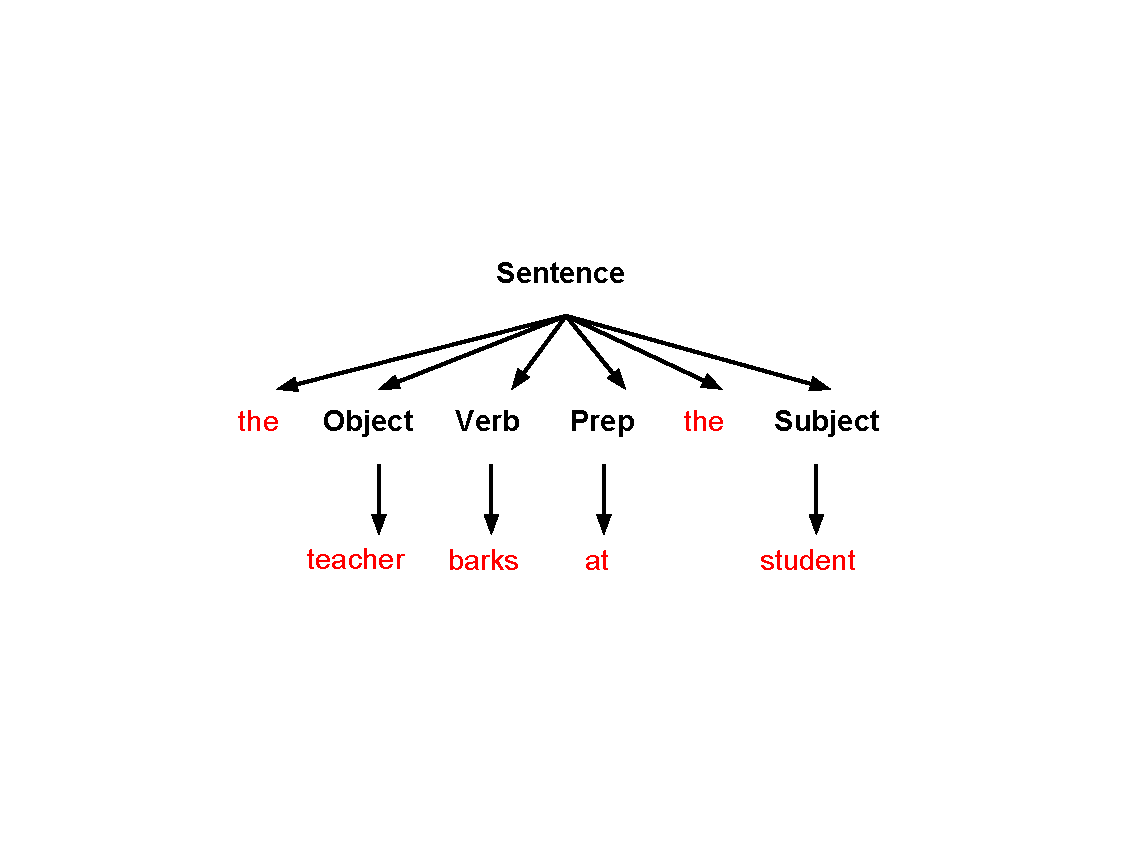
\includegraphics[width=12.5cm]{images/stree}  
\end{center}



\end{frame}

\begin{frame}[fragile]
\frametitle{Мета-език на Бекус-Наур}

\begin{itemize}
\item $<digit> ::= 0 | 1 | 2 | 3 | 4 | 5 | 6 | 7 | 8 | 9 $
\item $<unsigned int> ::= <digit>^+$
\item $<integer> ::= [+|-] <unsigned int>$
\item $<identifier> ::= \_ (<letter> | <digit> | \_ )^* | <leter> (<letter> | <digit> | \_ )^* $
\end{itemize}

\end{frame}


\end{document}


\begin{columns}[t]
  \begin{column}{0.2\textwidth}

  \end{column}
  \begin{column}{0.8\textwidth}

  \end{column}
\end{columns}


